\documentclass{article}

\usepackage[a4paper, margin=2cm]{geometry}
\usepackage[utf8]{inputenc}
\usepackage[T1]{fontenc}

\usepackage[czech]{babel}
\usepackage{fvextra}
\usepackage{csquotes}
\usepackage{parskip}

\usepackage{float}
\usepackage{amsmath}
\usepackage{siunitx}
\usepackage{graphicx}

\usepackage[hidelinks, unicode, pdfusetitle]{hyperref}

\DeclareMathOperator{\sign}{sign}

\graphicspath{{images}}

\title{Mnohoúhelník}
\author{Benjamin Swart}

\begin{document}

Bod leží uvnitř konvexního mnohoúhelníku, pokud leží na \enquote{správné} straně všech jeho hran, tj. na té, na které leží zbylé body mnohoúhelníka. Projdeme tedy všechny hrany a ověříme, jestli tomu tak je.

\begin{figure}[ht]
    \centering
    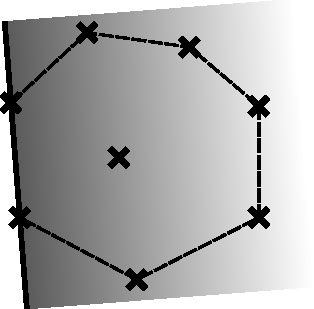
\includegraphics[scale=1.5]{polygon.pdf}
\end{figure}

Máme tedy body $p_1$ a $p_2$ určující úsečku, libovolný další bod mnohoúhelníka $q$ a bod $x$. Bod $p_1$ zvolíme jako počátek soustavy souřadnic a odečteme ho od ostatních bodů, čímž získáme vektory $p^\prime = p_2 - p_1$, $q^\prime = q - p_1$ a $v^\prime = x - p_1$.

Dále najdeme normalizovaný vektor kolmý na $p$, a to tak, že ho otočíme o devadesát stupňů a normalizujeme:

\begin{equation*}
    n = \frac{
        \begin{bmatrix}
            0 & -1 \\
            1 & 0
        \end{bmatrix} p^\prime
    }{||p^\prime||}
\end{equation*}

Poté určíme velikost projekce $q^\prime$ a $x^\prime$ na $n$ a porovnáme jejich znaménka:

\begin{equation*}
    \sign{\left<q^\prime, n\right>} = \sign{\left<x^\prime, n\right>}
\end{equation*}

Pokud tato rovnice neplatí, tak leží bod $x$ mimo daný mnohoúhelník. Pokud platí pro všechny úsečky, tak leží uvnitř. Pokud je $\left<q^\prime, n\right> = 0$, tak náš vstup obsahuje tři body ležící na jedné přímce, a protřední z nich redy není doopravdy vrcholem. Pokud chceme mít robustní algoritmus, tak ho můžeme odstranit.

Tento algoritmus má složitost $\mathcal{O}\left(n\right)$, protože mnohoúhelník s $n$ vrcholy má i $n$ úseček.

\end{document}
